% This is "sig-alternate.tex" V2.1 April 2013
% This file should be compiled with V2.5 of "sig-alternate.cls" May 2012
%
% This example file demonstrates the use of the 'sig-alternate.cls'
% V2.5 LaTeX2e document class file. It is for those submitting
% articles to ACM Conference Proceedings WHO DO NOT WISH TO
% STRICTLY ADHERE TO THE SIGS (PUBS-BOARD-ENDORSED) STYLE.
% The 'sig-alternate.cls' file will produce a similar-looking,
% albeit, 'tighter' paper resulting in, invariably, fewer pages.
%
% ----------------------------------------------------------------------------------------------------------------
% This .tex file (and associated .cls V2.5) produces:
%       1) The Permission Statement
%       2) The Conference (location) Info information
%       3) The Copyright Line with ACM data
%       4) NO page numbers
%
% as against the acm_proc_article-sp.cls file which
% DOES NOT produce 1) thru' 3) above.
%
% Using 'sig-alternate.cls' you have control, however, from within
% the source .tex file, over both the CopyrightYear
% (defaulted to 200X) and the ACM Copyright Data
% (defaulted to X-XXXXX-XX-X/XX/XX).
% e.g.
% \CopyrightYear{2007} will cause 2007 to appear in the copyright line.
% \crdata{0-12345-67-8/90/12} will cause 0-12345-67-8/90/12 to appear in the copyright line.
%
% ---------------------------------------------------------------------------------------------------------------
% This .tex source is an example which *does* use
% the .bib file (from which the .bbl file % is produced).
% REMEMBER HOWEVER: After having produced the .bbl file,
% and prior to final submission, you *NEED* to 'insert'
% your .bbl file into your source .tex file so as to provide
% ONE 'self-contained' source file.
%
% ================= IF YOU HAVE QUESTIONS =======================
% Questions regarding the SIGS styles, SIGS policies and
% procedures, Conferences etc. should be sent to
% Adrienne Griscti (griscti@acm.org)
%
% Technical questions _only_ to
% Gerald Murray (murray@hq.acm.org)
% ===============================================================
%
% For tracking purposes - this is V2.0 - May 2012

\documentclass{sig-alternate-05-2015}


\begin{document}

% Copyright
\setcopyright{acmcopyright}
%\setcopyright{acmlicensed}
%\setcopyright{rightsretained}
%\setcopyright{usgov}
%\setcopyright{usgovmixed}
%\setcopyright{cagov}
%\setcopyright{cagovmixed}


% DOI
\doi{10.475/123_4}

% ISBN
\isbn{123-4567-24-567/08/06}

%Conference
\conferenceinfo{PLDI '13}{June 16--19, 2013, Seattle, WA, USA}

\acmPrice{\$15.00}

%
% --- Author Metadata here ---
\conferenceinfo{WOODSTOCK}{'97 El Paso, Texas USA}
%\CopyrightYear{2007} % Allows default copyright year (20XX) to be over-ridden - IF NEED BE.
%\crdata{0-12345-67-8/90/01}  % Allows default copyright data (0-89791-88-6/97/05) to be over-ridden - IF NEED BE.
% --- End of Author Metadata ---

\title{BDA: A Platform for Big Data Analysis}
\subtitle{[Extended Abstract]
\titlenote{A full version of this paper is available as
\textit{Author's Guide to Preparing ACM SIG Proceedings Using
\LaTeX$2_\epsilon$\ and BibTeX} at
\texttt{www.acm.org/eaddress.htm}}}
%
% You need the command \numberofauthors to handle the 'placement
% and alignment' of the authors beneath the title.
%
% For aesthetic reasons, we recommend 'three authors at a time'
% i.e. three 'name/affiliation blocks' be placed beneath the title.
%
% NOTE: You are NOT restricted in how many 'rows' of
% "name/affiliations" may appear. We just ask that you restrict
% the number of 'columns' to three.
%
% Because of the available 'opening page real-estate'
% we ask you to refrain from putting more than six authors
% (two rows with three columns) beneath the article title.
% More than six makes the first-page appear very cluttered indeed.
%
% Use the \alignauthor commands to handle the names
% and affiliations for an 'aesthetic maximum' of six authors.
% Add names, affiliations, addresses for
% the seventh etc. author(s) as the argument for the
% \additionalauthors command.
% These 'additional authors' will be output/set for you
% without further effort on your part as the last section in
% the body of your article BEFORE References or any Appendices.

\numberofauthors{8} %  in this sample file, there are a *total*
% of EIGHT authors. SIX appear on the 'first-page' (for formatting
% reasons) and the remaining two appear in the \additionalauthors section.
%
\author{
% You can go ahead and credit any number of authors here,
% e.g. one 'row of three' or two rows (consisting of one row of three
% and a second row of one, two or three).
%
% The command \alignauthor (no curly braces needed) should
% precede each author name, affiliation/snail-mail address and
% e-mail address. Additionally, tag each line of
% affiliation/address with \affaddr, and tag the
% e-mail address with \email.
%
% 1st. author
\alignauthor
Ben Trovato\titlenote{Dr.~Trovato insisted his name be first.}\\
       \affaddr{Institute for Clarity in Documentation}\\
       \affaddr{1932 Wallamaloo Lane}\\
       \affaddr{Wallamaloo, New Zealand}\\
       \email{trovato@corporation.com}
% 2nd. author
\alignauthor
G.K.M. Tobin\titlenote{The secretary disavows
any knowledge of this author's actions.}\\
       \affaddr{Institute for Clarity in Documentation}\\
       \affaddr{P.O. Box 1212}\\
       \affaddr{Dublin, Ohio 43017-6221}\\
       \email{webmaster@marysville-ohio.com}
% 3rd. author
\alignauthor Lars Th{\o}rv{\"a}ld\titlenote{This author is the
one who did all the really hard work.}\\
       \affaddr{The Th{\o}rv{\"a}ld Group}\\
       \affaddr{1 Th{\o}rv{\"a}ld Circle}\\
       \affaddr{Hekla, Iceland}\\
       \email{larst@affiliation.org}
\and  % use '\and' if you need 'another row' of author names
% 4th. author
\alignauthor Lawrence P. Leipuner\\
       \affaddr{Brookhaven Laboratories}\\
       \affaddr{Brookhaven National Lab}\\
       \affaddr{P.O. Box 5000}\\
       \email{lleipuner@researchlabs.org}
% 5th. author
\alignauthor Sean Fogarty\\
       \affaddr{NASA Ames Research Center}\\
       \affaddr{Moffett Field}\\
       \affaddr{California 94035}\\
       \email{fogartys@amesres.org}
% 6th. author
\alignauthor Charles Palmer\\
       \affaddr{Palmer Research Laboratories}\\
       \affaddr{8600 Datapoint Drive}\\
       \affaddr{San Antonio, Texas 78229}\\
       \email{cpalmer@prl.com}
}
% There's nothing stopping you putting the seventh, eighth, etc.
% author on the opening page (as the 'third row') but we ask,
% for aesthetic reasons that you place these 'additional authors'
% in the \additional authors block, viz.
\additionalauthors{Additional authors: John Smith (The Th{\o}rv{\"a}ld Group,
email: {\texttt{jsmith@affiliation.org}}) and Julius P.~Kumquat
(The Kumquat Consortium, email: {\texttt{jpkumquat@consortium.net}}).}
\date{30 July 1999}
% Just remember to make sure that the TOTAL number of authors
% is the number that will appear on the first page PLUS the
% number that will appear in the \additionalauthors section.

\maketitle
\begin{abstract}
Big data processing and machine learning have made the world a better place. However, configuring machine learning task is always a complicated job. BDA is a GUI-based platform for big data analysis and mining, which provides a wealth of machine learning algorithms. Based on Hadoop and Spark, BDA is able to process massive datasets. One begins a task by construct dataflow based acyclic graph of algorithms with GUI. Each link in the acyclic graph represents a dataflow between algorithms. Machine learning is made easy, beautiful and understandable in BDA.
\end{abstract}


%
% The code below should be generated by the tool at
% http://dl.acm.org/ccs.cfm
% Please copy and paste the code instead of the example below. 
%
\begin{CCSXML}
<ccs2012>
 <concept>
  <concept_id>10010520.10010553.10010562</concept_id>
  <concept_desc>Computer systems organization~Embedded systems</concept_desc>
  <concept_significance>500</concept_significance>
 </concept>
 <concept>
  <concept_id>10010520.10010575.10010755</concept_id>
  <concept_desc>Computer systems organization~Redundancy</concept_desc>
  <concept_significance>300</concept_significance>
 </concept>
 <concept>
  <concept_id>10010520.10010553.10010554</concept_id>
  <concept_desc>Computer systems organization~Robotics</concept_desc>
  <concept_significance>100</concept_significance>
 </concept>
 <concept>
  <concept_id>10003033.10003083.10003095</concept_id>
  <concept_desc>Networks~Network reliability</concept_desc>
  <concept_significance>100</concept_significance>
 </concept>
</ccs2012>  
\end{CCSXML}

\ccsdesc[500]{Computer systems organization~Embedded systems}
\ccsdesc[300]{Computer systems organization~Redundancy}
\ccsdesc{Computer systems organization~Robotics}
\ccsdesc[100]{Networks~Network reliability}


%
% End generated code
%

%
%  Use this command to print the description
%
\printccsdesc

% We no longer use \terms command
%\terms{Theory}

\keywords{Data Mining; Big Data Analysis; Machine Learning}

\section{Introduction}
Data mining and analysis have been widely use in many industry verticals, such as financial services, communications, retail and e-commerce. However, configuring and going through the whole roadmap of data mining and analysis will be a complicated job. Integrated applications that facilitate going through the data mining and analysis job are widely demanded for data scientists and business analysts. 

Traditional tools like SAS, SPSS show their strength on descriptive and diagnostic analytics, and are useful for static structural datasets. However, they are not cloud-based, which limited the usage of advanced techniques in distributed systems. Systems like Azure Machine Learning and Alibaba Yushanfang are modern cloud platform for data scientists to design data experiments.

Modern analysis tools shares features, such as native support advanced analytic modeling techniques, visualization of dataflow design, ability to save dataflows into files and libraries for later reuse, allowing program using scripting language.

We present a modern cloud-based Big Data Analysis(BDA) system, which meets features described above. It's design on distributed system, Hadoop and Spark, and choose Oozie as job scheduler. 

\section{TECHNOLOGY SPECIFICATION}
\subsection{System Architecture}
BDA is a GUI-based platform designed on distributed system. It applied HDFS as storage, Spark and Map-Reduce as computation framework, and Oozie as job scheduler. Figure~\ref{fig:arch} shows system architecture.

\begin{figure}
\centering
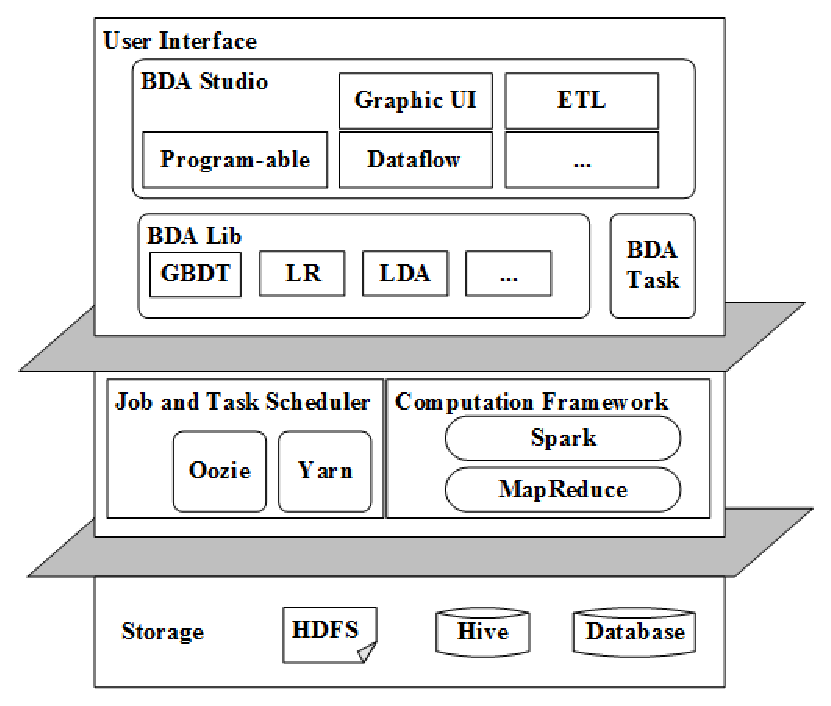
\includegraphics[height=2.8in]{cikm-architecture.eps}
\caption{ A overview of BDA architecture.}
\label{fig:arch}
\end{figure}

We divide the architecture into three hierarchy: Resource Management Layer, Schedule and Computation Layer and User Interface Layer.
\begin{itemize}
\item \textbf{Resource Management Layer:} This layer focuses on how to store the resources and datasets. We use database to store meta data of programs and jobs, while programs were stored on HDFS. All resources are stored on HDFS. And, Hive was applied to facilitates reading, writing, and managing large datasets residing in HDFS using SQL.
\item \textbf{Schedule and Computation Layer:} This layer focuses on how bda jobs are dispatched and executed. BDA applied Oozie as job scheduler. Each actions in the job will be dispatched to any node in the Haddop cluster by YARN and run as a Map task. Spark and Map-Reduce is our foundation of distributed computation framework.
\item \textbf{User Interface Layer:} This layer focuses how to provide friendly functionality for data scientists. There are three components, BDA Studio, BDA Lib and BDA Task. BDA Studio is a web service which support graphic-based components, program-able components, and dataflow based acyclic job graph constructions. BDA Lib provides a wealth of machine learning algorithms. BDA Task provides examples of real use cases.
\end{itemize}
We will introduce how these layer cooperation.


\section{BDA Lib}
BDA Lib is the algorithm library of BDA, it provides a wealth of machine learning, data mining algorithms. We have both Standalone and Spark implementations for each algorithm. All these algorithms are uploaded to BDA system and categorized as pre-processing, transformation, machine learning, and evaluation. Besides, we provide a sort of API for BDA Lib.

Each algorithm upload to BDA will be persist as a directory on HDFS, in which there are a run script of the algorithm, a directory named "lib". Run script is generated for algorithm to help start up the algorithm program. The directory "lib" contains all resources and executable files that are demand when the algorithm is used.

When uploading to BDA, the usage command line format of algorithm must be correctly configured. Otherwise, algorithm won't run successfully. The real command line would be generated when a BDA job is submitted, with configurations of algorithms. The command line format must be defined following the rules bellow:

\begin{itemize}
\item \textbf{For Input File Position Holder:}

 \{in:ContentType:"descriptions"\}
\item \textbf{For Output File Position Holder:}

\{out:ContentType,StorageType:"descriptions"\}
\item \textbf{For Numerical Parameter Position Holder:}

["parameter name":Type,min,max:default,value]
\item \textbf{For Boolean Parameter Position Holder:}

["parameter name":Bool:default,value]
\item \textbf{For String Parameter Position Holder:}

 ["parameter name":String:default,"value"]
\end{itemize}

ContentType specifies the format of file contents, where General as general files, LibSVM, TSV, CSV, Binary, JSON, XML.

StoreType specifies how the resources is store on HDFS, where SFile as a single file, HFile as a Hadoop distributed file, and Directory.

For numerical parameter, Type specifies the parameter types which may be Integer, Double or Float. In additions, the min and max value could be skipped if there are no minimum or maximum limitations.

Here comes an example of logistic regression(LR) command line format, it specifies the usage of LR train. $train\_pt$, $validate\_pt$, and $model\_pt$ are input files. $optimizer$, $max\_iter$, $reg$ and $learn\_rate$ are parameters of LR.

$$
\begin{array}{ll}
java~-cp~local.jar & bda.local.runnable.LR.Train \\
--train\_pt & \{in:LibSVM:"train~set"\}\\
--validate\_pt & \{in:LibSVM:"validate~set"\}\\
--model\_pt & \{out:Binary,HFile:"model"\}\\
--optimizer & ["opt":String:default,"sgd"]\\
--max\_iter & ["max\_iter":Integer:default,20]\\
--reg & ["reg":Double:default,0.01]\\
--learn\_rate & ["learn\_rate":Double:default,0.1]
\end{array}
$$


\section{BDA Studio}
BDA Studio is a GUI-based web service on the top of BDA architecture, allowed data scientists to access to resources and services provided by BDA easily. BDA Studio provides services like job schedule, distributed dispatch and execution, account management and resource management. 

\begin{figure}
\centering
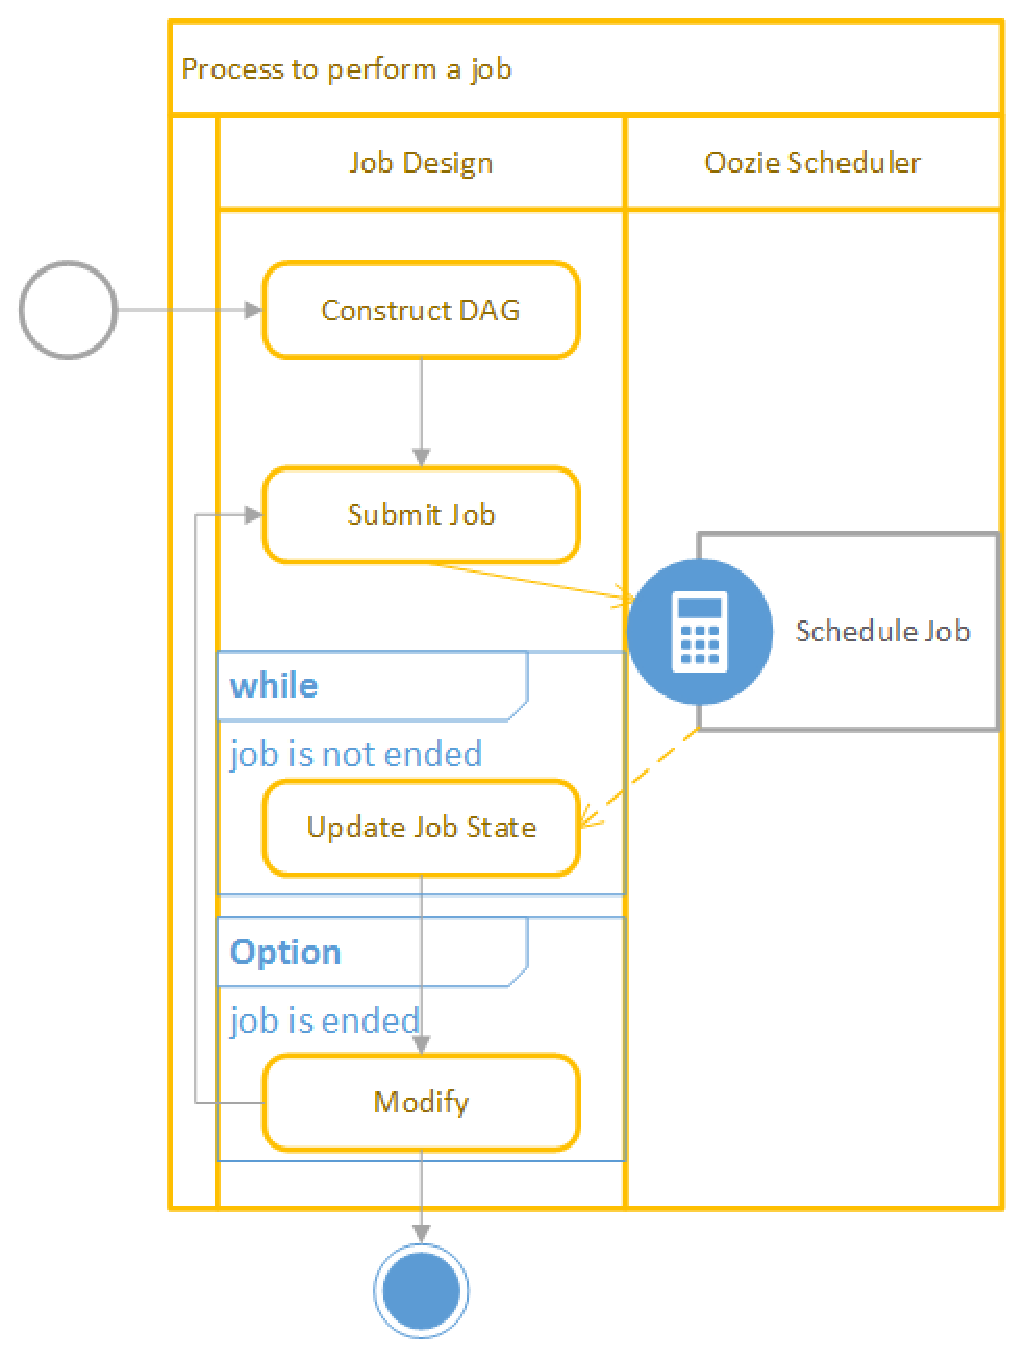
\includegraphics[height=3.5in]{proc.eps}
\caption{ Process to perform job.}
\label{fig:proc}
\end{figure}

Figure~\ref{fig:proc} shows the process to perform a job. As is shown, one must construct a dataflow based acyclic graph of algorithms and datasets, where each arrow specify a dataflow. When a well-formed job graph is submitted, it will be scheduled by Oozie, and finally run on the cloud. We also provide job clone, rerun and edit functionalities which facilitates the reuse of job schemas after the job is finished. 


The main technical challenges we have encountered are: GUI based DAG construction; dataflow based on Oozie workflow; enable program running on the cloud; ETL.

Besides, user custom programs are allowed to submit to the platform with configuration. In addition, BDA also provide program-able components, which support SQL, Spark, and Shell. 


\subsection{Dataflow Based Acyclic Graph}
We introduce dataflow based acyclic graph into BDA system based on Oozie workflow. And Oozie is a workflow scheduler system, where workflow is a collection of actions arranged in a control dependency DAG(Directed Acyclic Graph). Control dependency from one action to another means that the second action can't run until the first action has completed. The concept dataflow differed with workflow as to dataflow specify data dependency between different actions. And the control dependency of actions are determined by the data dependency.


\begin{figure}
\centering
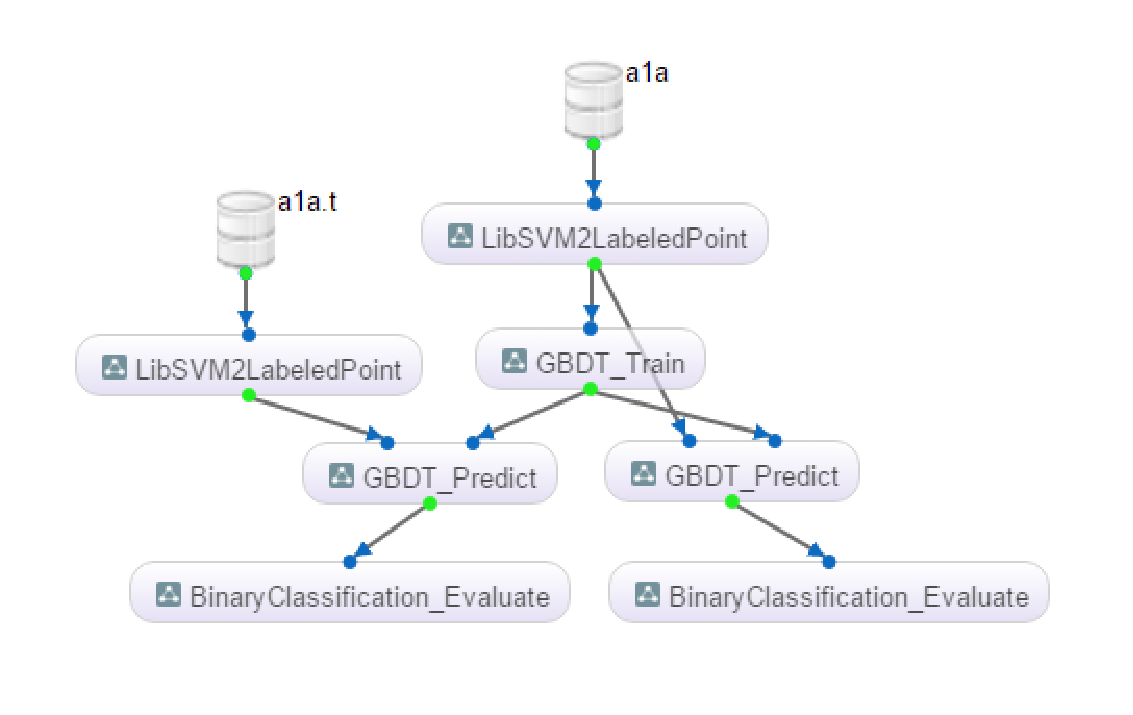
\includegraphics[height=2in]{DAG.eps}
\caption{ An example for dataflow based acyclic job graph.}
\label{fig:dag}
\end{figure}

Figure~\ref{fig:dag} is an example for dataflow based acyclic job graph. Each algorithm or dataset uploaded to BDA, will be represented as a GUI component in BDA Studio, where the points on the top of component are dataflow input anchor points and on the bottom are dataflow output anchor points. Anchor points are generated according to algorithm data parameters. Each arrow represent as a data dependency between components. In addition, the arrow's start and end anchor points must be matched, otherwise the algorithm will not run correctly.

\subsection{Run jobs on the cloud}

When the job graph is submitting, uuid file name will be created against each dataflow output anchor points. Later, the file parameter holder of the command format will be replaced with real file name according to setting of anchor points. In additions, other parameter holder will be replaced according to real parameter settings.

After the job is submitted, BDA Studio will generate Oozie workflow according to dataflow based acyclic job graph. And workflow will be upload to the job path created on HDFS. Finally, we will submit this job to Oozie server which 

Each Oozie action collected in the workflow will run as a Hadoop map task when it's scheduled. During the action, run script of respected algorithm will be sent to task container at first. Then run script will be started up. During the execution of the run script, it will configure the environment, download "lib" directory, execute the real command line, and upload file yielded to job path.

\subsection{Edit and reuse job schema}
BDA job, 数据重用等等.

\subsection{Program-able Component}
What’s program-able component?
It’s important to ETL. The significance of ETL.
The technology specification 

\section{Appendix}

\section{Conclusions}
This paragraph will end the body of this sample document.
Remember that you might still have Acknowledgments or
Appendices; brief samples of these
follow.  There is still the Bibliography to deal with; and
we will make a disclaimer about that here: with the exception
of the reference to the \LaTeX\ book, the citations in
this paper are to articles which have nothing to
do with the present subject and are used as
examples only.
%\end{document}  % This is where a 'short' article might terminate

%ACKNOWLEDGMENTS are optional
\section{Acknowledgments}
This section is optional; it is a location for you
to acknowledge grants, funding, editing assistance and
what have you.  In the present case, for example, the
authors would like to thank Gerald Murray of ACM for
his help in codifying this \textit{Author's Guide}
and the \textbf{.cls} and \textbf{.tex} files that it describes.

%
% The following two commands are all you need in the
% initial runs of your .tex file to
% produce the bibliography for the citations in your paper.
\bibliographystyle{abbrv}
\bibliography{sigproc}  % sigproc.bib is the name of the Bibliography in this case
% You must have a proper ".bib" file
%  and remember to run:
% latex bibtex latex latex
% to resolve all references
%
% ACM needs 'a single self-contained file'!
%
%APPENDICES are optional
%\balancecolumns
\appendix
%Appendix A
\section{Headings in Appendices}
The rules about hierarchical headings discussed above for
the body of the article are different in the appendices.
In the \textbf{appendix} environment, the command
\textbf{section} is used to
indicate the start of each Appendix, with alphabetic order
designation (i.e. the first is A, the second B, etc.) and
a title (if you include one).  So, if you need
hierarchical structure
\textit{within} an Appendix, start with \textbf{subsection} as the
highest level. Here is an outline of the body of this
document in Appendix-appropriate form:
\subsection{Introduction}
\subsection{The Body of the Paper}
\subsubsection{Type Changes and  Special Characters}
\subsubsection{Math Equations}
\paragraph{Inline (In-text) Equations}
\paragraph{Display Equations}
\subsubsection{Citations}
\subsubsection{Tables}
\subsubsection{Figures}
\subsubsection{Theorem-like Constructs}
\subsubsection*{A Caveat for the \TeX\ Expert}
\subsection{Conclusions}
\subsection{Acknowledgments}
\subsection{Additional Authors}
This section is inserted by \LaTeX; you do not insert it.
You just add the names and information in the
\texttt{{\char'134}additionalauthors} command at the start
of the document.
\subsection{References}
Generated by bibtex from your ~.bib file.  Run latex,
then bibtex, then latex twice (to resolve references)
to create the ~.bbl file.  Insert that ~.bbl file into
the .tex source file and comment out
the command \texttt{{\char'134}thebibliography}.
% This next section command marks the start of
% Appendix B, and does not continue the present hierarchy
\section{More Help for the Hardy}
The sig-alternate.cls file itself is chock-full of succinct
and helpful comments.  If you consider yourself a moderately
experienced to expert user of \LaTeX, you may find reading
it useful but please remember not to change it.
%\balancecolumns % GM June 2007
% That's all folks!
\end{document}
